\faQuestionCircle~Unsure about order of study one and two. Currently
chronological. But could also be: (1) main model works in larger student
sample, (2) works in economic migrant sample, (3) test full thing in
medical sample.

\section{Study 1}

Based on our main hypotheses, the aim of our first study is to
specifically test the general contact hypothesis, the influence of core
need fulfillment, and perceived interaction quality during intergroup
contacts. To this aim, we conducted an intensive longitudinal survey
study with recent migrants to the Netherlands, gathering a large body of
ecologically valid data on need satisfaction in real-life intergroup
contact situations. Data was collected from May 5th through June 6th,
2018 (and all participants started the study within the first two days).

The full surveys are available in our Online Supplementary Material A
and the full data description is available in Online Supplementary
Materials B. Correlations and descriptive statistics of the included
variables are available in Table \ref{tab:workerVarDescr} and Table
\ref{tab:workerOutVarDescr}.

\subsection{Methods}

\subsubsection{Participants}

After receiving ethical approval from the University of Groningen, we
recruited 23 migrants using the local paid participant pool and
specifically targeted non-Dutch migrants to participate in our study.
Participants reported on their interactions for at least 30 days with
two daily measures (capturing the morning and afternoon). With this
design, we aimed at getting 50-60 measurements per participant
(\textit{M} = 53.26, \textit{M} = 16.72, \textit{total N} = 1225). This
is a common number of measurements found in experience sampling studies
and should offer sufficient power to model processes within and between
participants \citep[e.g., for a systematic review see][]{AanhetRot2012}.
Participants were compensated for their participation with up to 34
Euros -- each two Euros for pre- and post-questionnaire as well as 50
Eurocents for every experience sampling measurement occasion. The sample
consisted of relatively young, educated, and western migrants from the
global north (\(M_{age}\) = 24.35, \(SD_{age}\) = 4.73, 19 women, 15
students). The sample accurately describes one of the largest groups of
migrants in the region \citep[][]{GemeenteGroningen2015}.

\subsubsection{Procedure}

The study itself consisted of three main parts, an introductory
pre-measurement, and the daily experience sampling measurements, as well
as a concluding post-measurement. After giving informed consent,
participants started by filling in an online pre-questionnaire assessing
demographics and general information about their immigration. Over the
next thirty days, the participants then were invited twice a day (at 12
pm and 7pm) to reflect upon their interactions, psychological need
fulfillments, and current attitudes towards the Dutch outgroup
(\textit{median duration} = 22, \textit{MAD duration} = 19). General
compliance was high (85.90\% of all invited surveys were filled
in)\footnote{Two participants completed only two days (among the others, participation was 93.70\%)}.
The response rates were approximately equal during mornings (\textit{n}
= 621) and afternoons (\textit{n} = 604) and most measurements were
completed within four hours of the invitation. After the final day of
daily diary measurements, participants were invited to fill in a longer
post measurement survey that mirrored the pre-measurement. All key
variables in for this study were part of the short daily diary surveys.

\subsubsection{Materials}

\paragraph{Intergroup Contact}

To test the prerequisite effect of intergroup contact, every experience
sampling measurement started with the question
``\textit{Did you meet a Dutch person this morning [/afternoon]? (In person interaction for at least 10 minutes)}''.
Our participants recorded between 2--51 (3.23--91.07\% of individual
daily diary measurements; 31.59\% of all 1225 daily diary
responses)\footnote{Two participants only recorded two daily diary measurements each and non of these included outgroup contacts. These participants are removed from any analyses including outgroup contacts.}.

\paragraph{Psychological Needs}

Irrespective of whether participants had an interaction with Dutch
people or not, everyone answered a short series of questions on
psychological need fulfillment. However, whereas participants with
interactions reported on the need fulfillment during the interaction,
people without interactions with Dutch people judged the past daytime
period in general. To assess the fulfillment of psychological needs, we
included two types of need measurement: (1) the core situational need
and (2) general self-determination theory needs.

For the core situational need, we asked participants in an open ended
text field:
``\textit{What was your most important goal [during the interaction / this morning / this afternoon]?}''.
Then, with reference to the text entry, we asked how much this core need
was fulfilled during the interaction or the past daytime period:
``\textit{[The interaction / you] fulfilled your goal: [-previous text entry-]}''
on a continuous slider scale ranging from strongly disagree (-50) to
strongly agree (+50).

We, additionally, included a common measure of three self-determination
theory needs \citep[see][]{Downie2008}. The items were introduced either
by ``\textit{During the interaction:}'' or
``\textit{This morning [/afternoon]:}'' and measured autonomy
(``\textit{I was myself.}''), competence
(``\textit{I felt competent.}''), and relatedness (without intergroup
contact ``\textit{I had a strong need to belong}''; with intergroup
contact: ``\textit{I shared information about myself.}'' and
``\textit{The other(s) shared information about themselves.}''). All
items were rated on a continuous slider scale from very little (-50) to
a great deal (+50).

\paragraph{Perceived Interaction Quality}

As an explanatory mechanism, we assessed ratings of the perceived
interaction quality. As our main measurement, participants rated the
statement ``\textit{Overall the interaction was …}'' on two continuous
slider scales measuring pleasantness
\citep[from unpleasant (-50) to pleasant (+50)) and meaningfulness (from superficial (-50) to meaningful (+50); both items adapted from][]{Downie2008}.

\paragraph{Outgroup Attitudes}

At the end of every daily diary measurement we asked all participants
about their current attitudes towards the Dutch -- our main dependent
variable. To assess the momentary outgroup evaluation we used the common
feeling thermometer: ``How favorable do you feel towards the Dutch?''
\citep[][]{Lavrakas2008}. Participants then rated their attitude on a
continuous slider scale from ``very cold -- 0'' through ``no feeling --
50'' to ``very warm -- 100''. Both the question phrasing as well as the
tick labels were consistent with large-scale panel surveys
\citep[e.g.,][]{DeBell2010}.

\begin{table}
\begin{minipage}[t][\textheight][t]{\textwidth}

\caption{\label{tab:workerVarDescr}Worker: Multilevel Core Variable Descriptives}
\centering
\resizebox{\linewidth}{!}{
\begin{tabular}[t]{llccccc}
\toprule
  & Core Need & Competence & Autonomy & Relatedness & Quality & Attitudes NL\\
\midrule
Core Need &  & 0.82*** & 0.60*** & 0.33 & 0.52** & -0.03\\
Competence & 0.36*** &  & 0.89*** & 0.26 & 0.39 & -0.23\\
Autonomy & 0.28*** & 0.22*** &  & 0.31 & 0.57** & 0.02\\
Relatedness & 0.50*** & 0.39*** & 0.37*** &  & -0.07 & 0.14\\
Quality & 0.17*** & 0.44*** & 0.27*** & 0.26*** &  & 0.50*\\
Attitudes NL & 0.24*** & 0.36*** & 0.24*** & 0.37*** & 0.52*** & \\
\addlinespace
Grand Mean & 27.95 & 12.10 & 22.17 & 5.29 & 24.10 & 71.49\\
Between SD & 14.68 & 13.72 & 12.09 & 14.59 & 9.50 & 12.91\\
Within SD & NA & NA & NA & NA & NA & NA\\
ICC(1) & 0.29 & 0.28 & 0.38 & 0.28 & 0.18 & 0.70\\
ICC(2) & 0.96 & 0.95 & 0.97 & 0.95 & 0.79 & 0.99\\
Within.person.SD & 20.83 & 20.89 & 15.15 & 23.29 & 18.01 & 8.11\\
\bottomrule
\multicolumn{7}{l}{\rule{0pt}{1em}\textit{Note: }}\\
\multicolumn{7}{l}{\rule{0pt}{1em}Upper triangle: Between-person correlations;}\\
\multicolumn{7}{l}{\rule{0pt}{1em}Lower triangle: Within-person correlations;}\\
\multicolumn{7}{l}{\rule{0pt}{1em}*** p < .001, ** p < .01,  * p < .05}\\
\end{tabular}}
\end{minipage}
\end{table}

\begin{table}
\begin{minipage}[t][\textheight][t]{\textwidth}

\caption{\label{tab:workerOutVarDescr}Worker: Multilevel Core Variable Descriptives (Outgroup Contact Only)}
\centering
\resizebox{\linewidth}{!}{
\begin{tabular}[t]{llcc}
\toprule
  & Core Need & Quality & Attitudes NL\\
\midrule
Core Need &  & 0.40 & -0.03\\
Quality & 0.37*** &  & 0.21\\
Attitudes NL & 0.27*** & 0.55*** & \\
\addlinespace
Grand Mean & 82.20 & 67.00 & 72.46\\
Between SD & 12.42 & 9.26 & 13.62\\
Within SD & 17.66 & 18.24 & 9.50\\
\addlinespace
ICC(1) & 0.33 & 0.23 & 0.68\\
ICC(2) & 0.90 & 0.84 & 0.98\\
\bottomrule
\multicolumn{4}{l}{\rule{0pt}{1em}\textit{Note: }}\\
\multicolumn{4}{l}{\rule{0pt}{1em}Upper triangle: Between-person correlations;}\\
\multicolumn{4}{l}{\rule{0pt}{1em}Lower triangle: Within-person correlations;}\\
\multicolumn{4}{l}{\rule{0pt}{1em}*** p < .001, ** p < .01,  * p < .05}\\
\end{tabular}}
\end{minipage}
\end{table}


\subsection{Results}

\begin{Shaded}
\begin{Highlighting}[]
\CommentTok{\# correlation panel}
\FunctionTok{pairs.panels.new}\NormalTok{(}
\NormalTok{  dtWorkerSupp}\SpecialCharTok{$}\NormalTok{workerAvFreQual }\SpecialCharTok{\%\textgreater{}\%} \FunctionTok{select}\NormalTok{(SumContactNL, SumContactNLAll, AvQuality, AvAttitude),}
  \AttributeTok{labels =} \FunctionTok{c}\NormalTok{(}
    \StringTok{"Sum:}\SpecialCharTok{\textbackslash{}n}\StringTok{Numer of beeps with Outgroup Contact (NL)"}\NormalTok{,}
    \StringTok{"Sum:}\SpecialCharTok{\textbackslash{}n}\StringTok{Number of Outgroup Contacts (NL)"}\NormalTok{,}
    \StringTok{"Mean:}\SpecialCharTok{\textbackslash{}n}\StringTok{Interaction Quality"}\NormalTok{,}
    \StringTok{"Mean:}\SpecialCharTok{\textbackslash{}n}\StringTok{Outgroup Attitudes (NL)"}
\NormalTok{  )}
\NormalTok{)}
\end{Highlighting}
\end{Shaded}

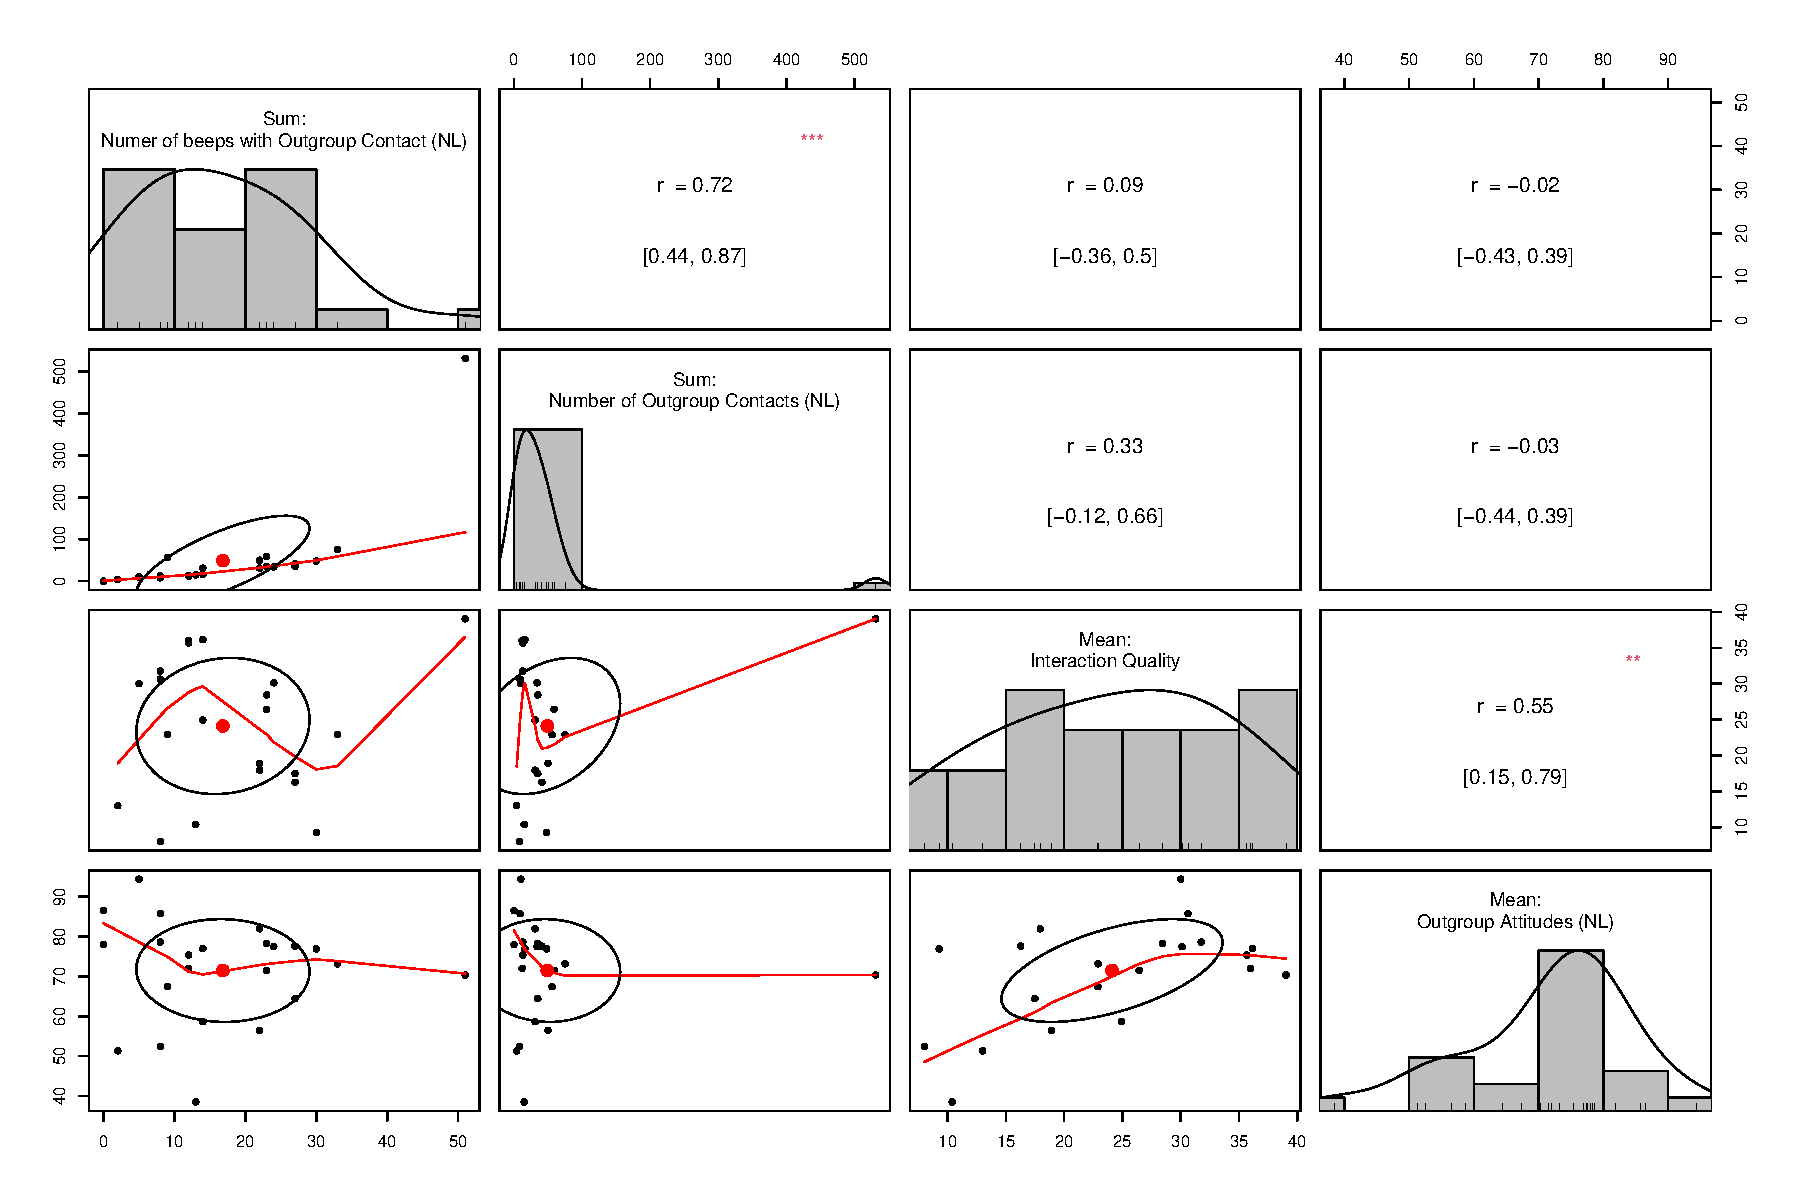
\includegraphics{Figures/WorkerFreqAttCor-1.pdf}

\begin{Shaded}
\begin{Highlighting}[]
\CommentTok{\# correlation panel with interaction sums winsorized}
\FunctionTok{pairs.panels.new}\NormalTok{(}
\NormalTok{  dtWorkerSupp}\SpecialCharTok{$}\NormalTok{workerAvFreQual }\SpecialCharTok{\%\textgreater{}\%} \FunctionTok{select}\NormalTok{(WinSumContactNL, WinSumContactNLAll, AvQuality, AvAttitude),}
  \AttributeTok{labels =} \FunctionTok{c}\NormalTok{(}
    \StringTok{"Sum:}\SpecialCharTok{\textbackslash{}n}\StringTok{Numer of beeps with Outgroup Contact (NL)}\SpecialCharTok{\textbackslash{}n}\StringTok{[Winsorized]"}\NormalTok{,}
    \StringTok{"Sum:}\SpecialCharTok{\textbackslash{}n}\StringTok{Number of Outgroup Contacts (NL)}\SpecialCharTok{\textbackslash{}n}\StringTok{[Winsorized]"}\NormalTok{,}
    \StringTok{"Mean:}\SpecialCharTok{\textbackslash{}n}\StringTok{Interaction Quality"}\NormalTok{,}
    \StringTok{"Mean:}\SpecialCharTok{\textbackslash{}n}\StringTok{Outgroup Attitudes (NL)"}
\NormalTok{  )}
\NormalTok{)}
\end{Highlighting}
\end{Shaded}

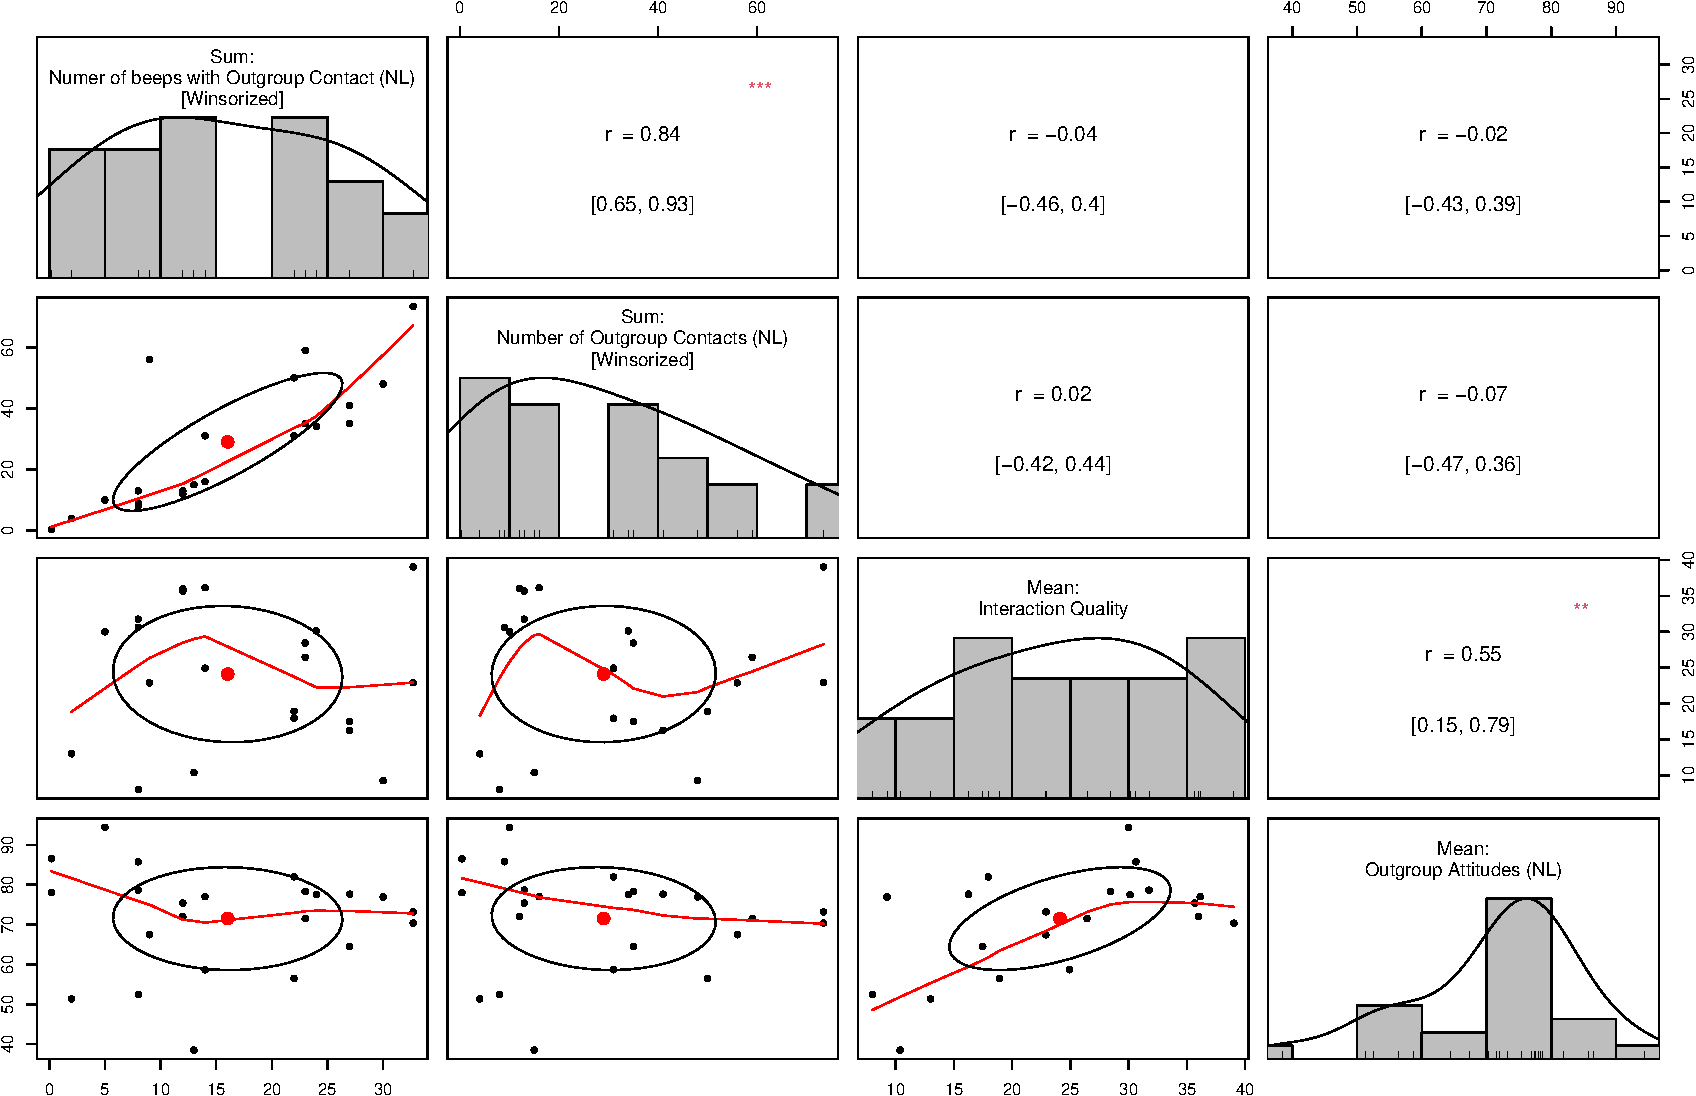
\includegraphics{Figures/WorkerFreqAttCor-2.pdf}

\paragraph{Contact Hypothesis}

We tested the most general contact hypothesis in two steps. First, we
assessed whether more intergroup interactions were related to to more
positive outgroup attitudes. Second, we tested whether a potential
positive effect on outgroup attitudes depended on the interaction
quality (jointly with the number of interactions). We find that neither
the number of interactions nor the number of daily diary responses with
an interaction were significantly related with the average outgroup
attitudes. This is to say that within our data, participants with more
outgroup interactions did not have significantly more positive outgroup
attitudes. This might be due to the aggregation within the participants
or the small sample size of between participant data. Nonetheless, the
aggregate data does not support the notion that simply having more
interactions with an outgroup results in more positive outgroup
attitudes.

\begin{Shaded}
\begin{Highlighting}[]
\CommentTok{\# create list to store Worker models}
\NormalTok{mdlWorker }\OtherTok{\textless{}{-}} \FunctionTok{list}\NormalTok{()}

\CommentTok{\# regression}
\NormalTok{mdlWorker}\SpecialCharTok{$}\NormalTok{lmAttFreqQualX }\OtherTok{\textless{}{-}}
  \FunctionTok{lm}\NormalTok{(AvAttitude }\SpecialCharTok{\textasciitilde{}}\NormalTok{ SumContactNL }\SpecialCharTok{*}\NormalTok{ AvQuality, }\AttributeTok{data =}\NormalTok{ dtWorkerSupp}\SpecialCharTok{$}\NormalTok{workerAvFreQual)}
\CommentTok{\# summary(lmWorkerAttFreqQualX)}

\FunctionTok{summ}\NormalTok{(}
\NormalTok{  mdlWorker}\SpecialCharTok{$}\NormalTok{lmAttFreqQualX,}
  \AttributeTok{confint =} \ConstantTok{TRUE}\NormalTok{,}
  \AttributeTok{digits =} \DecValTok{3}\NormalTok{,}
  \AttributeTok{center =} \ConstantTok{TRUE}
\NormalTok{)}
\end{Highlighting}
\end{Shaded}

\begin{table}[!h]
\centering
\begin{tabular}{lr}
\toprule
\cellcolor{gray!6}{Observations} & \cellcolor{gray!6}{21 (2 missing obs. deleted)}\\
Dependent variable & AvAttitude\\
\cellcolor{gray!6}{Type} & \cellcolor{gray!6}{OLS linear regression}\\
\bottomrule
\end{tabular}
\end{table} \begin{table}[!h]
\centering
\begin{tabular}{lr}
\toprule
\cellcolor{gray!6}{F(3,17)} & \cellcolor{gray!6}{6.663}\\
R² & 0.540\\
\cellcolor{gray!6}{Adj. R²} & \cellcolor{gray!6}{0.459}\\
\bottomrule
\end{tabular}
\end{table} \begin{table}[!h]
\centering
\begin{threeparttable}
\begin{tabular}{lrrrrr}
\toprule
  & Est. & 2.5\% & 97.5\% & t val. & p\\
\midrule
\cellcolor{gray!6}{(Intercept)} & \cellcolor{gray!6}{70.930} & \cellcolor{gray!6}{66.519} & \cellcolor{gray!6}{75.341} & \cellcolor{gray!6}{33.927} & \cellcolor{gray!6}{0.000}\\
SumContactNL & 0.269 & -0.150 & 0.688 & 1.354 & 0.193\\
\cellcolor{gray!6}{AvQuality} & \cellcolor{gray!6}{0.765} & \cellcolor{gray!6}{0.288} & \cellcolor{gray!6}{1.242} & \cellcolor{gray!6}{3.385} & \cellcolor{gray!6}{0.004}\\
SumContactNL:AvQuality & -0.049 & -0.085 & -0.014 & -2.954 & 0.009\\
\bottomrule
\end{tabular}
\begin{tablenotes}
\item Standard errors: OLS; Continuous predictors are mean-centered.
\end{tablenotes}
\end{threeparttable}
\end{table}

\begin{Shaded}
\begin{Highlighting}[]
\NormalTok{mdlWorker}\SpecialCharTok{$}\NormalTok{lmAttFreqQualXEta }\OtherTok{\textless{}{-}}
\NormalTok{  effectsize}\SpecialCharTok{::}\FunctionTok{eta\_squared}\NormalTok{(mdlWorker}\SpecialCharTok{$}\NormalTok{lmAttFreqQualX, }\AttributeTok{partial =} \ConstantTok{TRUE}\NormalTok{)}

\NormalTok{interactions}\SpecialCharTok{::}\FunctionTok{interact\_plot}\NormalTok{(}
\NormalTok{  mdlWorker}\SpecialCharTok{$}\NormalTok{lmAttFreqQualX,}
  \AttributeTok{pred =}\NormalTok{ AvQuality,}
  \AttributeTok{modx =}\NormalTok{ SumContactNL,}
  \AttributeTok{interval =} \ConstantTok{TRUE}\NormalTok{,}
  \AttributeTok{partial.residuals =} \ConstantTok{TRUE}
\NormalTok{)}
\end{Highlighting}
\end{Shaded}

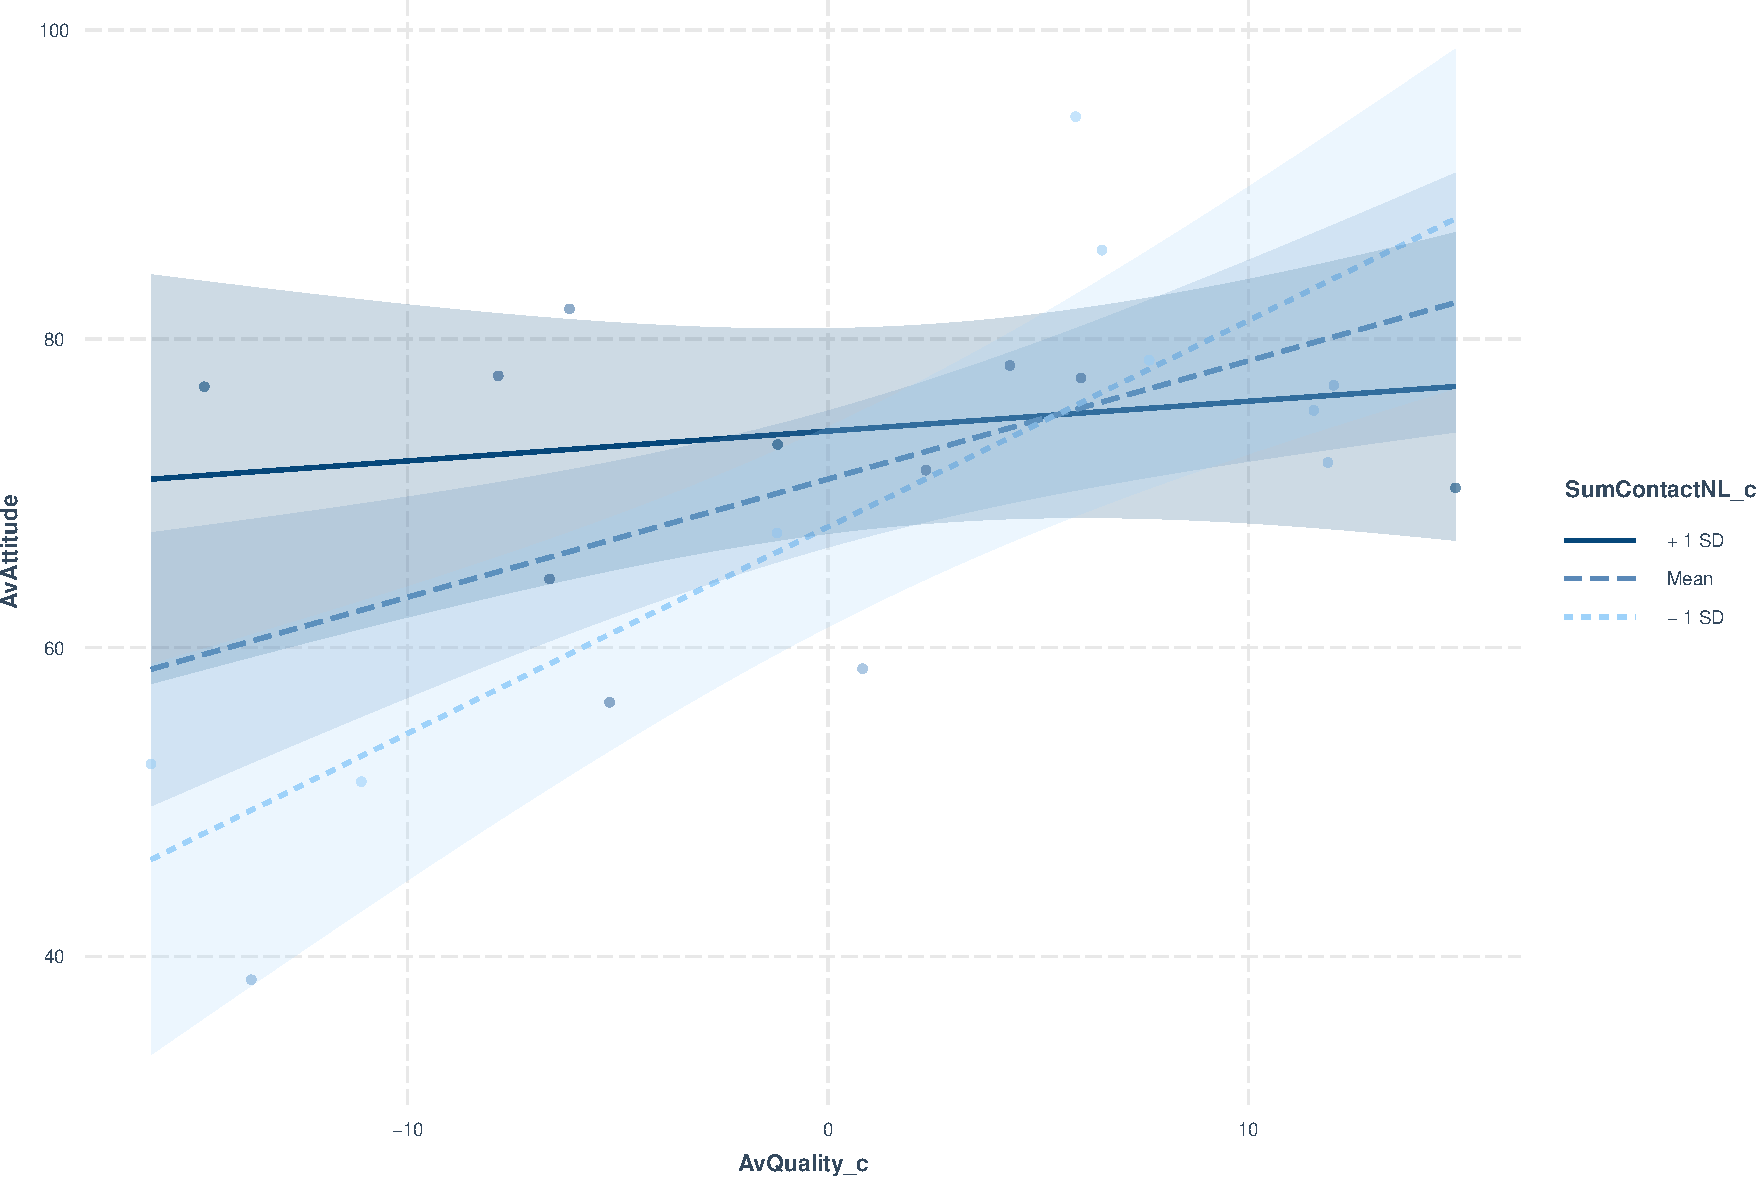
\includegraphics{Figures/workerModelOlsAttFreqQual-1.pdf}

\begin{Shaded}
\begin{Highlighting}[]
\NormalTok{interactions}\SpecialCharTok{::}\FunctionTok{johnson\_neyman}\NormalTok{(mdlWorker}\SpecialCharTok{$}\NormalTok{lmAttFreqQualX,}
                             \AttributeTok{pred =}\NormalTok{ AvQuality,}
                             \AttributeTok{modx =}\NormalTok{ SumContactNL,}
                             \AttributeTok{alpha =}\NormalTok{ .}\DecValTok{05}\NormalTok{)}
\end{Highlighting}
\end{Shaded}

\begin{verbatim}
## JOHNSON-NEYMAN INTERVAL 
## 
## When SumContactNL is OUTSIDE the interval [23.66, 75.42], the slope of AvQuality is p < .05.
## 
## Note: The range of observed values of SumContactNL is [2.00, 51.00]
\end{verbatim}

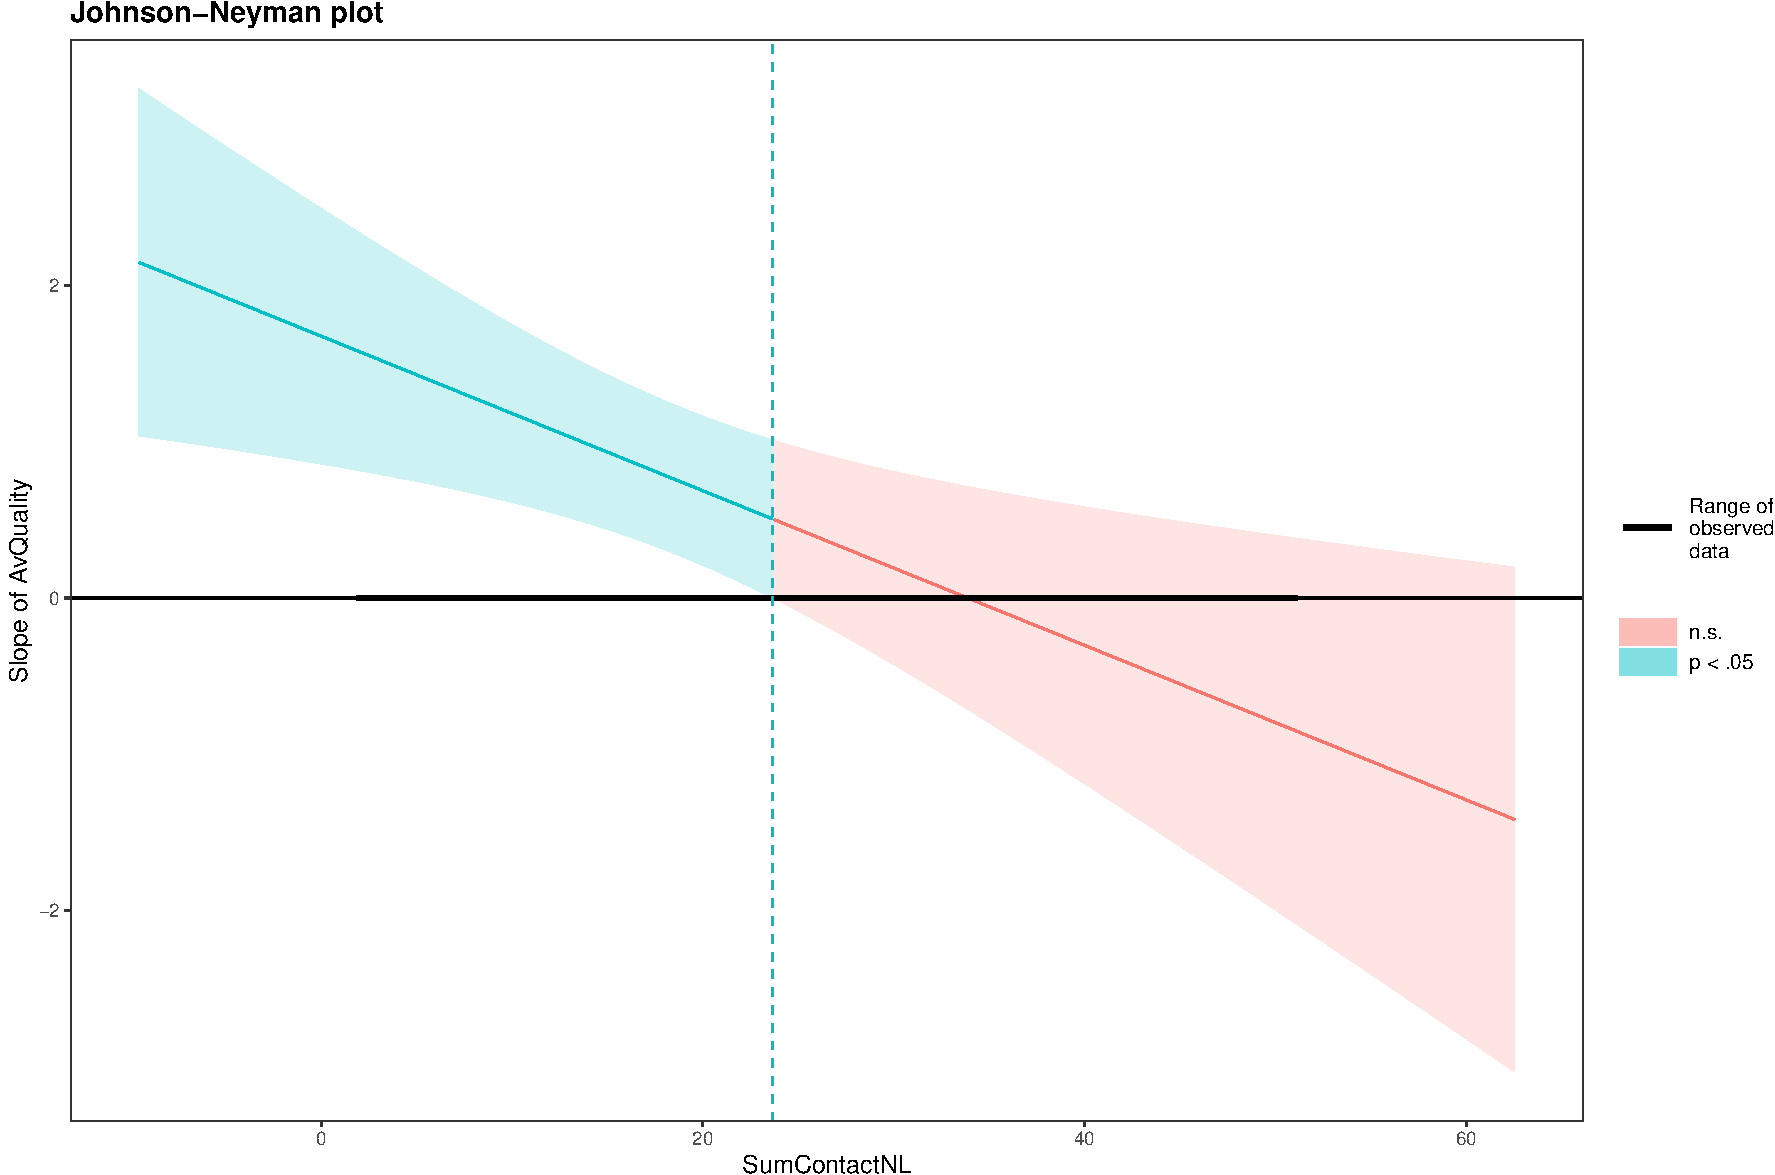
\includegraphics{Figures/workerModelOlsAttFreqQual-2.pdf}

However, despite the missing relationship with the number of
interactions, we find a medium sized correlation between the
participants' Average Interaction Quality and their Average Outgroup
Attitudes. Thus within our data participants with a higher quality
outgroup interactions also held more positive attitudes towards that
group. And when considering the number of interactions and average
interaction quality jointly in a linear regression, we additionally find
a statistically significant interaction term (\textit{b} = -0.05,
\textit{t}(17) = -2.95, \textit{p} = 0.009, \(\eta_p^2\) = 0.34).
Looking at a floodlight analysis of the effect, we find that in our
sample with an increasing number of interactions the positive effect of
average interaction quality becomes weaker. However, it should be noted
that this is based on data aggregating all within participant nuances
and is only the date of 21 people.

\begin{Shaded}
\begin{Highlighting}[]
\CommentTok{\# Create and save Model}
\NormalTok{mdlWorker}\SpecialCharTok{$}\NormalTok{lmerAttNull }\OtherTok{\textless{}{-}}
\NormalTok{  lme4}\SpecialCharTok{::}\FunctionTok{lmer}\NormalTok{(thermometerDutch\_1 }\SpecialCharTok{\textasciitilde{}} \DecValTok{1} \SpecialCharTok{+}\NormalTok{ (}\DecValTok{1} \SpecialCharTok{|}\NormalTok{ PID),}
    \AttributeTok{data =}\NormalTok{ dtWorker}\SpecialCharTok{$}\NormalTok{full}
\NormalTok{  ) }\CommentTok{\# use optim if it does not converge}

\NormalTok{mdlWorker}\SpecialCharTok{$}\NormalTok{lmeAttNull }\OtherTok{\textless{}{-}}
  \FunctionTok{lme}\NormalTok{(}
\NormalTok{    thermometerDutch\_1 }\SpecialCharTok{\textasciitilde{}} \DecValTok{1}\NormalTok{,}
    \AttributeTok{random =} \SpecialCharTok{\textasciitilde{}} \DecValTok{1} \SpecialCharTok{|}\NormalTok{ PID,}
    \AttributeTok{data =}\NormalTok{ dtWorker}\SpecialCharTok{$}\NormalTok{full,}
    \AttributeTok{control =} \FunctionTok{list}\NormalTok{(}\AttributeTok{opt =} \StringTok{"nlmimb"}\NormalTok{)}
\NormalTok{  ) }\CommentTok{\# use optim if it does not converge}

\CommentTok{\# Get summary with p{-}values (Satterthwaite\textquotesingle{}s method)}
\CommentTok{\# summary(lmerWorkerAttNull) \#or with the lme function}
\FunctionTok{summ}\NormalTok{(mdlWorker}\SpecialCharTok{$}\NormalTok{lmerAttNull, }\AttributeTok{digits =} \DecValTok{3}\NormalTok{, }\AttributeTok{center =} \ConstantTok{TRUE}\NormalTok{)}
\end{Highlighting}
\end{Shaded}

\begin{table}[!h]
\centering
\begin{tabular}{lr}
\toprule
\cellcolor{gray!6}{Observations} & \cellcolor{gray!6}{1225}\\
Dependent variable & thermometerDutch\_1\\
\cellcolor{gray!6}{Type} & \cellcolor{gray!6}{Mixed effects linear regression}\\
\bottomrule
\end{tabular}
\end{table} \begin{table}[!h]
\centering
\begin{tabular}{lr}
\toprule
\cellcolor{gray!6}{AIC} & \cellcolor{gray!6}{8805.880}\\
BIC & 8821.213\\
\cellcolor{gray!6}{Pseudo-R² (fixed effects)} & \cellcolor{gray!6}{0.000}\\
Pseudo-R² (total) & 0.698\\
\bottomrule
\end{tabular}
\end{table} \begin{table}[!h]
\centering
\begin{threeparttable}
\begin{tabular}{lrrrrr}
\toprule
\multicolumn{6}{c}{Fixed Effects} \\
\cmidrule(l{3pt}r{3pt}){1-6}
  & Est. & S.E. & t val. & d.f. & p\\
\midrule
\cellcolor{gray!6}{(Intercept)} & \cellcolor{gray!6}{71.338} & \cellcolor{gray!6}{2.695} & \cellcolor{gray!6}{26.466} & \cellcolor{gray!6}{22.053} & \cellcolor{gray!6}{0.000}\\
\bottomrule
\end{tabular}
\begin{tablenotes}
\item  p values calculated using Satterthwaite d.f. ; Continuous predictors are mean-centered.
\end{tablenotes}
\end{threeparttable}
\end{table} \begin{table}[!h]
\centering
\begin{tabular}{lll}
\toprule
\multicolumn{3}{c}{Random Effects} \\
\cmidrule(l{3pt}r{3pt}){1-3}
Group & Parameter & Std. Dev.\\
\midrule
\cellcolor{gray!6}{PID} & \cellcolor{gray!6}{(Intercept)} & \cellcolor{gray!6}{12.797}\\
Residual &  & 8.425\\
\bottomrule
\end{tabular}
\end{table} \begin{table}[!h]
\centering
\begin{tabular}{lrl}
\toprule
\multicolumn{3}{c}{Grouping Variables} \\
\cmidrule(l{3pt}r{3pt}){1-3}
Group & \# groups & ICC\\
\midrule
\cellcolor{gray!6}{PID} & \cellcolor{gray!6}{23} & \cellcolor{gray!6}{0.698}\\
\bottomrule
\end{tabular}
\end{table}

\begin{Shaded}
\begin{Highlighting}[]
\CommentTok{\# generate 95\% parametric bootstrap CIs (and save them as a csv{-}file):}
\CommentTok{\# write.csv(confint(lmer(thermometerDutch\_1\textasciitilde{}1 + (1|PID),data=dtWorker$full),}
\CommentTok{\#                  method="boot",nsim=1000,}
\CommentTok{\#                  parallel = "multicore", ncpus = 4, seed = 42),}
\CommentTok{\#          "output/tables/ML{-}Null{-}CI.csv")}

\CommentTok{\# Save variances}
\NormalTok{mdlWorker}\SpecialCharTok{$}\NormalTok{varAttNull }\OtherTok{\textless{}{-}} 
  \FunctionTok{VarCorr}\NormalTok{(mdlWorker}\SpecialCharTok{$}\NormalTok{lmeAttNull) }\CommentTok{\# save variances}
\CommentTok{\# The estimate of (between{-}group or Intercept variance, tau\_\{00\}\^{}2):}
\NormalTok{mdlWorker}\SpecialCharTok{$}\NormalTok{tauAttNull }\OtherTok{\textless{}{-}} 
  \FunctionTok{as.numeric}\NormalTok{(mdlWorker}\SpecialCharTok{$}\NormalTok{varAttNull[}\DecValTok{1}\NormalTok{])}
\CommentTok{\# and the estimate of (within{-}group or residual variance, sigma\^{}2) is:}
\NormalTok{mdlWorker}\SpecialCharTok{$}\NormalTok{sigmaAttNull }\OtherTok{\textless{}{-}} 
  \FunctionTok{as.numeric}\NormalTok{(mdlWorker}\SpecialCharTok{$}\NormalTok{varAttNull[}\DecValTok{2}\NormalTok{])}
\CommentTok{\# The ICC estimate (between/between+within) is:}
\NormalTok{mdlWorker}\SpecialCharTok{$}\NormalTok{IccAttNull }\OtherTok{\textless{}{-}}
\NormalTok{  (}\FunctionTok{as.numeric}\NormalTok{(mdlWorker}\SpecialCharTok{$}\NormalTok{varAttNull[}\DecValTok{1}\NormalTok{]) }\SpecialCharTok{/}\NormalTok{ (}\FunctionTok{as.numeric}\NormalTok{(mdlWorker}\SpecialCharTok{$}\NormalTok{varAttNull[}\DecValTok{1}\NormalTok{]) }\SpecialCharTok{+} \FunctionTok{as.numeric}\NormalTok{(mdlWorker}\SpecialCharTok{$}\NormalTok{varAttNull[}\DecValTok{2}\NormalTok{])))}
\NormalTok{mdlWorker}\SpecialCharTok{$}\NormalTok{IccPercAttNull }\OtherTok{\textless{}{-}}
\NormalTok{  ((}\FunctionTok{as.numeric}\NormalTok{(mdlWorker}\SpecialCharTok{$}\NormalTok{varAttNull[}\DecValTok{1}\NormalTok{]) }\SpecialCharTok{/}\NormalTok{ (}\FunctionTok{as.numeric}\NormalTok{(mdlWorker}\SpecialCharTok{$}\NormalTok{varAttNull[}\DecValTok{1}\NormalTok{]) }\SpecialCharTok{+} \FunctionTok{as.numeric}\NormalTok{(mdlWorker}\SpecialCharTok{$}\NormalTok{varAttNull[}\DecValTok{2}\NormalTok{])))) }\SpecialCharTok{*} \DecValTok{100}
\end{Highlighting}
\end{Shaded}

\begin{Shaded}
\begin{Highlighting}[]
\CommentTok{\# Create and save Model}
\NormalTok{mdlWorker}\SpecialCharTok{$}\NormalTok{lmeInterceptAttType }\OtherTok{\textless{}{-}}
  \FunctionTok{lme}\NormalTok{(}
\NormalTok{    thermometerDutch\_1 }\SpecialCharTok{\textasciitilde{}}\NormalTok{ OutgroupInteraction }\SpecialCharTok{+}\NormalTok{ NonOutgroupInteraction,}
    \AttributeTok{random =}  \SpecialCharTok{\textasciitilde{}} \DecValTok{1} \SpecialCharTok{|}\NormalTok{ PID,}
    \AttributeTok{data =}\NormalTok{ dtWorkerSupp}\SpecialCharTok{$}\NormalTok{workerInteractionType}
\NormalTok{  )}

\CommentTok{\# Get summary with p{-}values (Satterthwaite\textquotesingle{}s method)}
\FunctionTok{summ}\NormalTok{(}
\NormalTok{  mdlWorker}\SpecialCharTok{$}\NormalTok{lmerInterceptAttType }\OtherTok{\textless{}{-}} \FunctionTok{lmer}\NormalTok{(}
\NormalTok{    thermometerDutch\_1 }\SpecialCharTok{\textasciitilde{}}\NormalTok{ OutgroupInteraction }\SpecialCharTok{+}\NormalTok{ NonOutgroupInteraction }\SpecialCharTok{+}\NormalTok{ (}\DecValTok{1} \SpecialCharTok{|}\NormalTok{ PID),}
    \AttributeTok{data =}\NormalTok{ dtWorkerSupp}\SpecialCharTok{$}\NormalTok{workerInteractionType}
\NormalTok{  ),}
  \AttributeTok{confint =} \ConstantTok{TRUE}\NormalTok{,}
  \AttributeTok{digits =} \DecValTok{3}\NormalTok{,}
  \AttributeTok{center =} \ConstantTok{FALSE}
\NormalTok{)}
\end{Highlighting}
\end{Shaded}

\begin{table}[!h]
\centering
\begin{tabular}{lr}
\toprule
\cellcolor{gray!6}{Observations} & \cellcolor{gray!6}{1225}\\
Dependent variable & thermometerDutch\_1\\
\cellcolor{gray!6}{Type} & \cellcolor{gray!6}{Mixed effects linear regression}\\
\bottomrule
\end{tabular}
\end{table} \begin{table}[!h]
\centering
\begin{tabular}{lr}
\toprule
\cellcolor{gray!6}{AIC} & \cellcolor{gray!6}{8788.218}\\
BIC & 8813.771\\
\cellcolor{gray!6}{Pseudo-R² (fixed effects)} & \cellcolor{gray!6}{0.006}\\
Pseudo-R² (total) & 0.703\\
\bottomrule
\end{tabular}
\end{table} \begin{table}[!h]
\centering
\begin{threeparttable}
\begin{tabular}{lrrrrrr}
\toprule
\multicolumn{7}{c}{Fixed Effects} \\
\cmidrule(l{3pt}r{3pt}){1-7}
  & Est. & 2.5\% & 97.5\% & t val. & d.f. & p\\
\midrule
\cellcolor{gray!6}{(Intercept)} & \cellcolor{gray!6}{70.343} & \cellcolor{gray!6}{65.002} & \cellcolor{gray!6}{75.683} & \cellcolor{gray!6}{25.814} & \cellcolor{gray!6}{22.897} & \cellcolor{gray!6}{0.000}\\
OutgroupInteractionYes & 2.477 & 1.364 & 3.589 & 4.365 & 1204.135 & 0.000\\
\cellcolor{gray!6}{NonOutgroupInteractionyes} & \cellcolor{gray!6}{0.427} & \cellcolor{gray!6}{-0.683} & \cellcolor{gray!6}{1.538} & \cellcolor{gray!6}{0.754} & \cellcolor{gray!6}{1204.911} & \cellcolor{gray!6}{0.451}\\
\bottomrule
\end{tabular}
\begin{tablenotes}
\item  p values calculated using Satterthwaite d.f. 
\end{tablenotes}
\end{threeparttable}
\end{table} \begin{table}[!h]
\centering
\begin{tabular}{lll}
\toprule
\multicolumn{3}{c}{Random Effects} \\
\cmidrule(l{3pt}r{3pt}){1-3}
Group & Parameter & Std. Dev.\\
\midrule
\cellcolor{gray!6}{PID} & \cellcolor{gray!6}{(Intercept)} & \cellcolor{gray!6}{12.811}\\
Residual &  & 8.362\\
\bottomrule
\end{tabular}
\end{table} \begin{table}[!h]
\centering
\begin{tabular}{lrl}
\toprule
\multicolumn{3}{c}{Grouping Variables} \\
\cmidrule(l{3pt}r{3pt}){1-3}
Group & \# groups & ICC\\
\midrule
\cellcolor{gray!6}{PID} & \cellcolor{gray!6}{23} & \cellcolor{gray!6}{0.701}\\
\bottomrule
\end{tabular}
\end{table}

\begin{Shaded}
\begin{Highlighting}[]
\NormalTok{mdlWorker}\SpecialCharTok{$}\NormalTok{lmerInterceptAttTypeCI }\OtherTok{\textless{}{-}} \FunctionTok{confint}\NormalTok{(mdlWorker}\SpecialCharTok{$}\NormalTok{lmerInterceptAttType)}

\CommentTok{\# Generate 95\% parametric bootstrap CIs (and save them as a csv{-}file):}
\CommentTok{\# write.csv(confint(lmer(thermometerDutch\_1 \textasciitilde{} Contact\_dum + inNonDutch + (1|PID),data=dtWorker$full),}
\CommentTok{\#                  method="boot",nsim=1000, parallel = "multicore",}
\CommentTok{\#                  ncpus = 4, seed = 42),}
\CommentTok{\#          "output/tables/ML{-}Inter{-}CI.csv")}

\CommentTok{\# Compare new model to previous step}
\FunctionTok{anova}\NormalTok{(mdlWorker}\SpecialCharTok{$}\NormalTok{lmeAttNull, }
\NormalTok{      mdlWorker}\SpecialCharTok{$}\NormalTok{lmeInterceptAttType) }\SpecialCharTok{\%\textgreater{}\%}
  \FunctionTok{as.data.frame}\NormalTok{() }\SpecialCharTok{\%\textgreater{}\%}
  \FunctionTok{select}\NormalTok{(}\SpecialCharTok{{-}}\NormalTok{call) }\SpecialCharTok{\%\textgreater{}\%}
  \FunctionTok{mutate}\NormalTok{(}
    \AttributeTok{L.Ratio =} \FunctionTok{round}\NormalTok{(L.Ratio, }\DecValTok{3}\NormalTok{),}
    \StringTok{\textasciigrave{}}\AttributeTok{p{-}value}\StringTok{\textasciigrave{}} \OtherTok{=} \FunctionTok{ifelse}\NormalTok{(}\StringTok{\textasciigrave{}}\AttributeTok{p{-}value}\StringTok{\textasciigrave{}}\SpecialCharTok{\textgreater{}=}\NormalTok{.}\DecValTok{001}\NormalTok{, }\FunctionTok{round}\NormalTok{(}\StringTok{\textasciigrave{}}\AttributeTok{p{-}value}\StringTok{\textasciigrave{}}\NormalTok{, }\DecValTok{3}\NormalTok{), }\StringTok{"\textless{} .001"}\NormalTok{)}
\NormalTok{  ) }\SpecialCharTok{\%\textgreater{}\%}
  \FunctionTok{replace}\NormalTok{(}\FunctionTok{is.na}\NormalTok{(.), }\StringTok{""}\NormalTok{) }\SpecialCharTok{\%\textgreater{}\%}
  \FunctionTok{add\_rownames}\NormalTok{(., }\AttributeTok{var =} \StringTok{"Description"}\NormalTok{) }\SpecialCharTok{\%\textgreater{}\%}
  \FunctionTok{mutate}\NormalTok{(}\AttributeTok{Description =} \FunctionTok{gsub}\NormalTok{(}\StringTok{".*}\SpecialCharTok{\textbackslash{}\textbackslash{}}\StringTok{$"}\NormalTok{, }\StringTok{""}\NormalTok{, Description)) }\SpecialCharTok{\%\textgreater{}\%}
  \FunctionTok{kbl}\NormalTok{(}
\NormalTok{    .,}
    \AttributeTok{caption =} \StringTok{"Worker: Model Comparison"}\NormalTok{,}
    \AttributeTok{format =} \StringTok{"latex"}\NormalTok{,}
    \AttributeTok{linesep =} \StringTok{""}\NormalTok{,}
    \AttributeTok{booktabs =}\NormalTok{ T,}
    \AttributeTok{align =} \FunctionTok{rep}\NormalTok{(}\StringTok{"c"}\NormalTok{, }\FunctionTok{ncol}\NormalTok{(.)),}
    \AttributeTok{digits =} \DecValTok{3}
\NormalTok{  ) }\SpecialCharTok{\%\textgreater{}\%}
  \FunctionTok{kable\_styling}\NormalTok{(}\AttributeTok{position =} \StringTok{"left"}\NormalTok{)}
\end{Highlighting}
\end{Shaded}

\begin{table}

\caption{\label{tab:workerModelInterceptAttType}Worker: Model Comparison}
\begin{tabular}[t]{ccccccccc}
\toprule
Description & Model & df & AIC & BIC & logLik & Test & L.Ratio & p-value\\
\midrule
lmeAttNull & 1 & 3 & 8806 & 8821 & -4400 &  &  & \\
lmeInterceptAttType & 2 & 5 & 8788 & 8814 & -4389 & 1 vs 2 & 21.663 & < .001\\
\bottomrule
\end{tabular}
\end{table}

\begin{Shaded}
\begin{Highlighting}[]
\CommentTok{\# Save variances}
\NormalTok{mdlWorker}\SpecialCharTok{$}\NormalTok{varInterceptAttType }\OtherTok{\textless{}{-}} 
\NormalTok{  lme4}\SpecialCharTok{::}\FunctionTok{VarCorr}\NormalTok{(mdlWorker}\SpecialCharTok{$}\NormalTok{lmeInterceptAttType)}

\CommentTok{\# The estimate of between{-}group (or Intercept variance) explained:}
\CommentTok{\# Variance Explained = 1 – (Var with Predictor/Var without Predictor)}
\NormalTok{mdlWorker}\SpecialCharTok{$}\NormalTok{varBtwInterceptAttType }\OtherTok{\textless{}{-}}
  \DecValTok{1} \SpecialCharTok{{-}}\NormalTok{ (}\FunctionTok{as.numeric}\NormalTok{(mdlWorker}\SpecialCharTok{$}\NormalTok{varInterceptAttType[}\DecValTok{1}\NormalTok{]) }\SpecialCharTok{/} \FunctionTok{as.numeric}\NormalTok{(mdlWorker}\SpecialCharTok{$}\NormalTok{varAttNull[}\DecValTok{1}\NormalTok{]))}
\NormalTok{mdlWorker}\SpecialCharTok{$}\NormalTok{varBtwPercInterceptAttType }\OtherTok{\textless{}{-}}
\NormalTok{  (}\DecValTok{1} \SpecialCharTok{{-}}\NormalTok{ (}\FunctionTok{as.numeric}\NormalTok{(mdlWorker}\SpecialCharTok{$}\NormalTok{varInterceptAttType[}\DecValTok{1}\NormalTok{]) }\SpecialCharTok{/} \FunctionTok{as.numeric}\NormalTok{(mdlWorker}\SpecialCharTok{$}\NormalTok{varAttNull[}\DecValTok{1}\NormalTok{]))) }\SpecialCharTok{*} \DecValTok{100}
\CommentTok{\# and the estimate of within{-}group (or residual variance) explained is:}
\NormalTok{mdlWorker}\SpecialCharTok{$}\NormalTok{varWithinInterceptAttType }\OtherTok{\textless{}{-}}
  \DecValTok{1} \SpecialCharTok{{-}}\NormalTok{ (}\FunctionTok{as.numeric}\NormalTok{(mdlWorker}\SpecialCharTok{$}\NormalTok{varInterceptAttType[}\DecValTok{2}\NormalTok{]) }\SpecialCharTok{/} \FunctionTok{as.numeric}\NormalTok{(mdlWorker}\SpecialCharTok{$}\NormalTok{varAttNull[}\DecValTok{2}\NormalTok{]))}
\NormalTok{mdlWorker}\SpecialCharTok{$}\NormalTok{varWithinPercInterceptAttType }\OtherTok{\textless{}{-}}
\NormalTok{  (}\DecValTok{1} \SpecialCharTok{{-}}\NormalTok{ (}\FunctionTok{as.numeric}\NormalTok{(mdlWorker}\SpecialCharTok{$}\NormalTok{varInterceptAttType[}\DecValTok{2}\NormalTok{]) }\SpecialCharTok{/} \FunctionTok{as.numeric}\NormalTok{(mdlWorker}\SpecialCharTok{$}\NormalTok{varAttNull[}\DecValTok{2}\NormalTok{]))) }\SpecialCharTok{*} \DecValTok{100}
\end{Highlighting}
\end{Shaded}

We additionally used a multilevel regression to check whether having an
interaction with an outgroup member had a situational (i.e.,
contemporaneous) effect within the participants. We find that having an
outgroup interaction is indeed associated with significantly more
positive outgroup attitudes within the participants (\textit{b} = 2.48,
\textit{t}(1200) = 4.36, \textit{p} \textless{} .001,
\textit{95\%CI}{[}1.3644, 3.5884{]}), even after controlling for having
an interaction with a non-Dutch (which did not relate to outgroup
attitudes independently; For full results see Online Supplementary
Materials B).

\paragraph{Core Need}

\begin{itemize}
\tightlist
\item
  Att \textasciitilde{} Need \& Qlt \textasciitilde{} Need
\item
  Att \textasciitilde{} Need + Qual
\end{itemize}

\paragraph{Robustness}

\section{Study 2}

\subsection{Methods}

\subsection{Results}

\section{Study 2}

\subsection{Methods}

\subsection{Results}
